\chapter{Experimental Setup} 

\label{experimental_setup} 
% maybe name it considerations of pipeline design or something like this

% should contain
% pipeline architecture
% genus/strain/species
% strain+species

\section{Design considerations}
One of the main goals of this master thesis was to design a Nextflow pipeline performing reproducible machine learning. 
There are some research questions which influence the design choices taken.
With MetaPhlAn3 and kraken2 two different taxonomic profilers have been implemented. Other taxonomic profilers could be added in the future as well. This flexibility enables potential users to chose the best fitting profiler for their task or experiment if unsure.

Another important aspect is the taxonomic level on which the ML algorithm is learning its patterns. Depending on the illness genus, species, strain or a combination of species and strain is the more important. The user can decide which of these levels to looked at, or even use all of the above in order to learn which the most distinguishing levels for a certain illness are.

There are different ML algorithms implemented. The user can chose between SVM, RF, XG-Boost and L2-Linear Regression or take a multiple of them. 
% mention L2?
A feature selection can be indicated with its corresponding threshold value. The metric on which the algorithm optimizes is customizable. 
% can be chosen? MCC, balanced accuracy as sensible defaults


\section{Pipeline architecture}


\begin{figure}
	\centering
	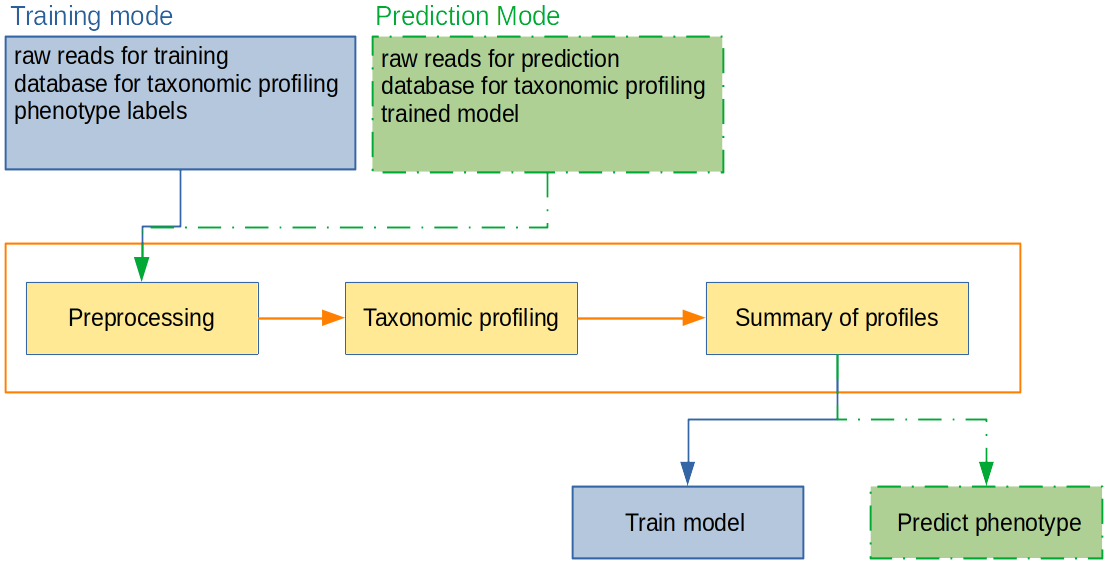
\includegraphics[width=0.9\textwidth]{Figures/pipeline_schemata_rev}
	%\decoRule
	\caption{Schema of the pipeline architecture. Train mode is blue colored, predict mode is green and the shared components are colored yellow.}
	\label{fig:schema}
\end{figure}


The Nextflow pipeline developed within this master thesis takes metagenomic data as input and trains a phenotype prediction algorithm with this information. It then can be used on unseen data for prediction.
Figure \ref{fig:schema} shows a schematic overview of the underlying architecture. 
% Train / predict mode
The pipeline has two distinct modes: training and prediction. Both modes share a common processing steps. Reads are trimmed based on their quality, host contamination is removed, taxonomic profiling is performed and summarized.

% how is the pipeline executed, example with paramters and flags

\subsection{Preprocessing}
Quality based trimming is performed with fastp \citep{fastp}. The 3'-end and the 5'-end are trimmed if the quality score in a sliding window falls below a preset threshold. Fastp is executed with these parameters:
\\
\code{fastp -q mean\_quality -{}-cut\_by\_quality5 -{}-cut\_by\_quality3 -{}-cut\_mean\_quality trimming\_quality}
\\
The quality score in the sliding window is set with the pipeline parameters \code{trimming\_quality} and \code{mean\_quality} which have a default value of 15.\\
% -M, --cut_mean_quality               the mean quality requirement option shared by cut_front, cut_tail or cut_sliding. Range: 1~36 default: 20 (Q20) (int [=20])
% -q, --qualified_quality_phred      the quality value that a base is qualified. Default 15 means phred quality >=Q15 is qualified. (int [=15])

% process in nextflow pipeline, should i mention it?

If host DNA is present it can be removed with bowtie2 \citep{bowtie2}.
To achieve this a fasta file of the host has to be provided. bowtie2 then finds and removes matches of the host DNA in the samples.

\subsection{Taxonomic profiling}
% mpa, kraken
By default both MetaPhlAn3 and kraken2 are used for taxonomic profiling. 
\code{-{}-skip\_metaphlan} and \code{-{}-skip\_kraken2} can be specified on pipeline execution when just one profiler is wished.
The databases are downloaded and configured automatically. If they are already present on the executing system their path can be specified with \code{-{}-kraken2\_db "\$PATH"} or \code{-{}-metaphlan\_db "\$PATH"} where \code{"\$PATH"} is a placeholder for the database path on the executing machine.

% execution with default parameters, can be changed

For each taxonomic profiler a summary table of all sample profiles is created with a custom python script using the pandas framework \citep{pandas}.

\subsection{Training mode}

% feature selection here

% data splitting for cv
% python script using scikit-learn
Figure \ref{fig:trainsplit} shows the data splitting scheme which is used during training mode. A custom python script uses the previously created summary table of taxonomic profiles to train the specified classifiers. All of the classifiers are implemented either in the scikit-learn or XGBoost packages.

% report of runtime and mean evaluation values
Finally mean values of ROC, (Balanced) Accuracy, Precision, Recall, F1-Score and MCC are reported together with the runtime. The trained classifiers are pickled and saved so that they can be used in the prediction mode. 

\begin{figure}
	\centering
	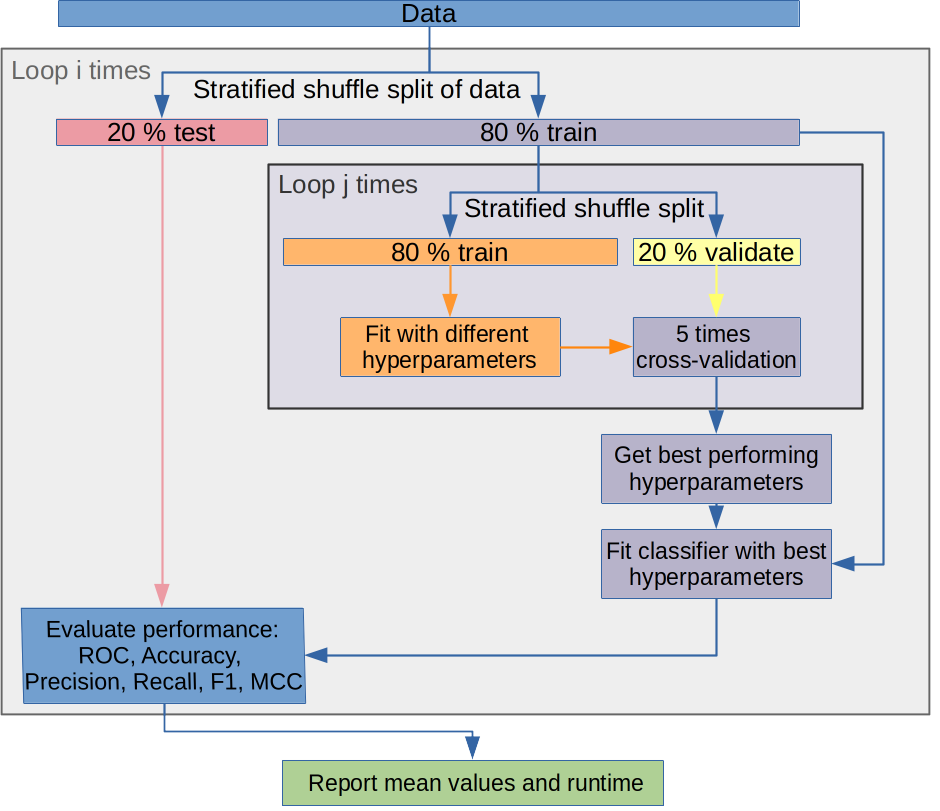
\includegraphics[width=0.9\textwidth]{Figures/ml_evaluation_datasplit_rev}
	%\decoRule
	\caption{Data splitting schema for testing and training. A stratified shuffle split is performed i-times on all of the data, respectively putting 20\% into the testing and 80\% in training set. Each training set is split j-times into 20\% validation and 80\% hyperparameter-training set. Five times cross-validation is used with this validation and training set to get the best performing hyperparameters. The performance then is evaluated i-times on the original test/train splits. Mean values and runtime are reported.}
	\label{fig:trainsplit}
\end{figure}


\subsection{Prediction mode}
% what class are the samples belonging to
For prediction mode one or more pretrained classifiers and the samples have to be provided. The same preprocessing and taxonomic profiling which has been used in training mode is performed on the samples. For the classification a python script uses the summary table of the taxonomic profiles and the classifiers yielding a prediction. 


% moved from results
\section{Datasets}

%which ones have been used, selection process, number of samples etc
There are several benchmark datasets which have been used for phenotype prediction.  Liver cirrhosis has yielded very good results before. Obesity is a hard case as researchers have struggled to get good performing predictions. Inflammatory Bowel Disease (IBD) is used as a smaller and imbalanced dataset yielding promising results. The number of samples and the size of the datasets is shown in table \ref{tab:datasets}. 


\begin{table}[]
	\centering
	\caption{Cases and sample size of considered datasets. Their size is given in Terabasepairs.}
	\label{tab:datasets}
	\begin{tabular}{lllll}
		\hline
		& Disease Cases & Healthy Cases & Total Samples & Size {[}Tbp{]} \\ \hline
		Liver Cirrhosis & 123     & 114    & 237   & 1.2            \\
		Obesity         & 169     & 123    & 292   & 1.6            \\
		IBD             & 25      & 99     & 124   & 0.39           \\ \hline
	\end{tabular}
\end{table}
